% =====================================================================
%  شرح مبسّط خطوة بخطوة: نمذجة وتحكم سلسلة طاقة ريحية PMSG 2 MW
%  التجميع: xelatex cours_PMSG.tex  (مرتين)
% =====================================================================
\documentclass[11pt,a4paper]{article}
\usepackage[margin=2.2cm]{geometry}
\usepackage{amsmath,amssymb}
\usepackage{graphicx}
\usepackage{booktabs}
\usepackage{xcolor}
\usepackage[framemethod=default]{mdframed}
\usepackage{fontspec}
\usepackage{hyperref}
\hypersetup{hidelinks}
\usepackage{polyglossia}
\setmainlanguage[numerals=maghrib]{arabic}
\setotherlanguage{french}
\setmainfont{Latin Modern Roman}
\newfontfamily\arabicfont[Script=Arabic,Scale=1.15]{Amiri}
\newfontfamily\arabicfontsf[Script=Arabic,Scale=1.15]{Amiri}
\newfontfamily\arabicfonttt[Script=Arabic,Scale=1.15]{Amiri}
\graphicspath{{figures/}}

\newcommand{\fr}[1]{\textfrench{#1}}
\newcommand{\bv}[1]{\boldsymbol{#1}}
\definecolor{fondA}{RGB}{232,242,252}
\definecolor{fondB}{RGB}{255,244,229}
\definecolor{fondC}{RGB}{236,247,232}
% صناديق: فكرة، مثال رقمي، تلخيص
\newmdenv[backgroundcolor=fondA,linecolor=blue!50!black,linewidth=0.8pt,innertopmargin=6pt,innerbottommargin=6pt]{fikra}
\newmdenv[backgroundcolor=fondB,linecolor=orange!70!black,linewidth=0.8pt,innertopmargin=6pt,innerbottommargin=6pt]{mithal}
\newmdenv[backgroundcolor=fondC,linecolor=green!40!black,linewidth=0.8pt,innertopmargin=6pt,innerbottommargin=6pt]{khulasa}
\newcommand{\Fikra}{\textbf{الفكرة: }}
\newcommand{\Mithal}{\textbf{مثال رقمي: }}
\newcommand{\Khulasa}{\textbf{الخلاصة: }}

\title{\textbf{شرح مبسّط خطوة بخطوة}\\[3mm]
\large نمذجة سلسلة طاقة ريحية بمولّد متزامن ذي مغانط دائمة (\fr{PMSG}) قدرتها \fr{2 MW}\\
والتحكم فيها بـ: التسطيح (\fr{platitude}) + السلبية (\fr{passivité}) + شبكة عصبونية (\fr{ANN})}
\author{سعيد رقاني — مخبر \fr{L2EI}، جامعة جيجل}
\date{}

\begin{document}
\maketitle

\begin{fikra}
\textbf{كيف تقرأ هذا الملف؟}
هذا الملف مكتوب لطالب لا يعرف شيئاً عن التحكم ولا عن الشبكات العصبونية. نبدأ من الصفر، ونشرح كل
معادلة: من أين جاءت، وماذا يعني كل حدّ فيها، ثم نعطي مثالاً بالأرقام الحقيقية لنظامنا.
المصطلحات التقنية مكتوبة بالفرنسية بين قوسين لأنها هي المستعملة في المقالات وفي البرامج.
الصناديق الزرقاء فيها \textbf{الفكرة}، والبرتقالية فيها \textbf{مثال رقمي}، والخضراء فيها \textbf{الخلاصة}.
\end{fikra}

\tableofcontents
\newpage

% =====================================================================
\section{الصورة الكبيرة: ماذا يفعل النظام؟}
% =====================================================================

النظام يحوّل \textbf{طاقة الريح} إلى \textbf{كهرباء} تُحقن في الشبكة الكهربائية. الطاقة تمرّ عبر سلسلة
من العناصر، وكل عنصر يحوّلها من شكل إلى آخر:

\begin{center}
\begin{tabular}{ccl}
\toprule
العنصر & يأخذ & ويعطي\\
\midrule
التوربينة (\fr{turbine}) & ريح & دوران (عزم \fr{$T_w$})\\
المولّد (\fr{PMSG}) & دوران & تيار متناوب بتردد متغيّر\\
المقوّم (\fr{redresseur MLI}) & تيار متناوب & تيار مستمر\\
الحافلة المستمرة (\fr{bus DC}) & تيار مستمر & يخزّن الطاقة مؤقتاً (مكثّف)\\
المموّج (\fr{onduleur MLI}) & تيار مستمر & تيار متناوب \fr{50 Hz}\\
المرشّح (\fr{filtre L}) & تيار متقطّع & تيار نظيف\\
الشبكة (\fr{réseau 690 V}) & --- & تستقبل الطاقة\\
\bottomrule
\end{tabular}
\end{center}

\paragraph{لماذا «\fr{back-to-back}»؟}
لأن المقوّم والمموّج موصولان «ظهراً لظهر» عبر الحافلة المستمرة. هذا يفصل المولّد عن الشبكة:
المولّد يدور بسرعة متغيّرة (حسب الريح)، والشبكة تبقى دائماً على \fr{50 Hz}.

\paragraph{لماذا «\fr{attaque directe}» (دفع مباشر)؟}
المولّد مركّب مباشرة على محور التوربينة، بدون علبة سرعات (\fr{multiplicateur}). لهذا يدور ببطء
(حوالي \fr{2 rad/s}) ويحتاج عدداً كبيراً من الأقطاب (\fr{26} زوجاً).

\begin{figure}[h]
\centering
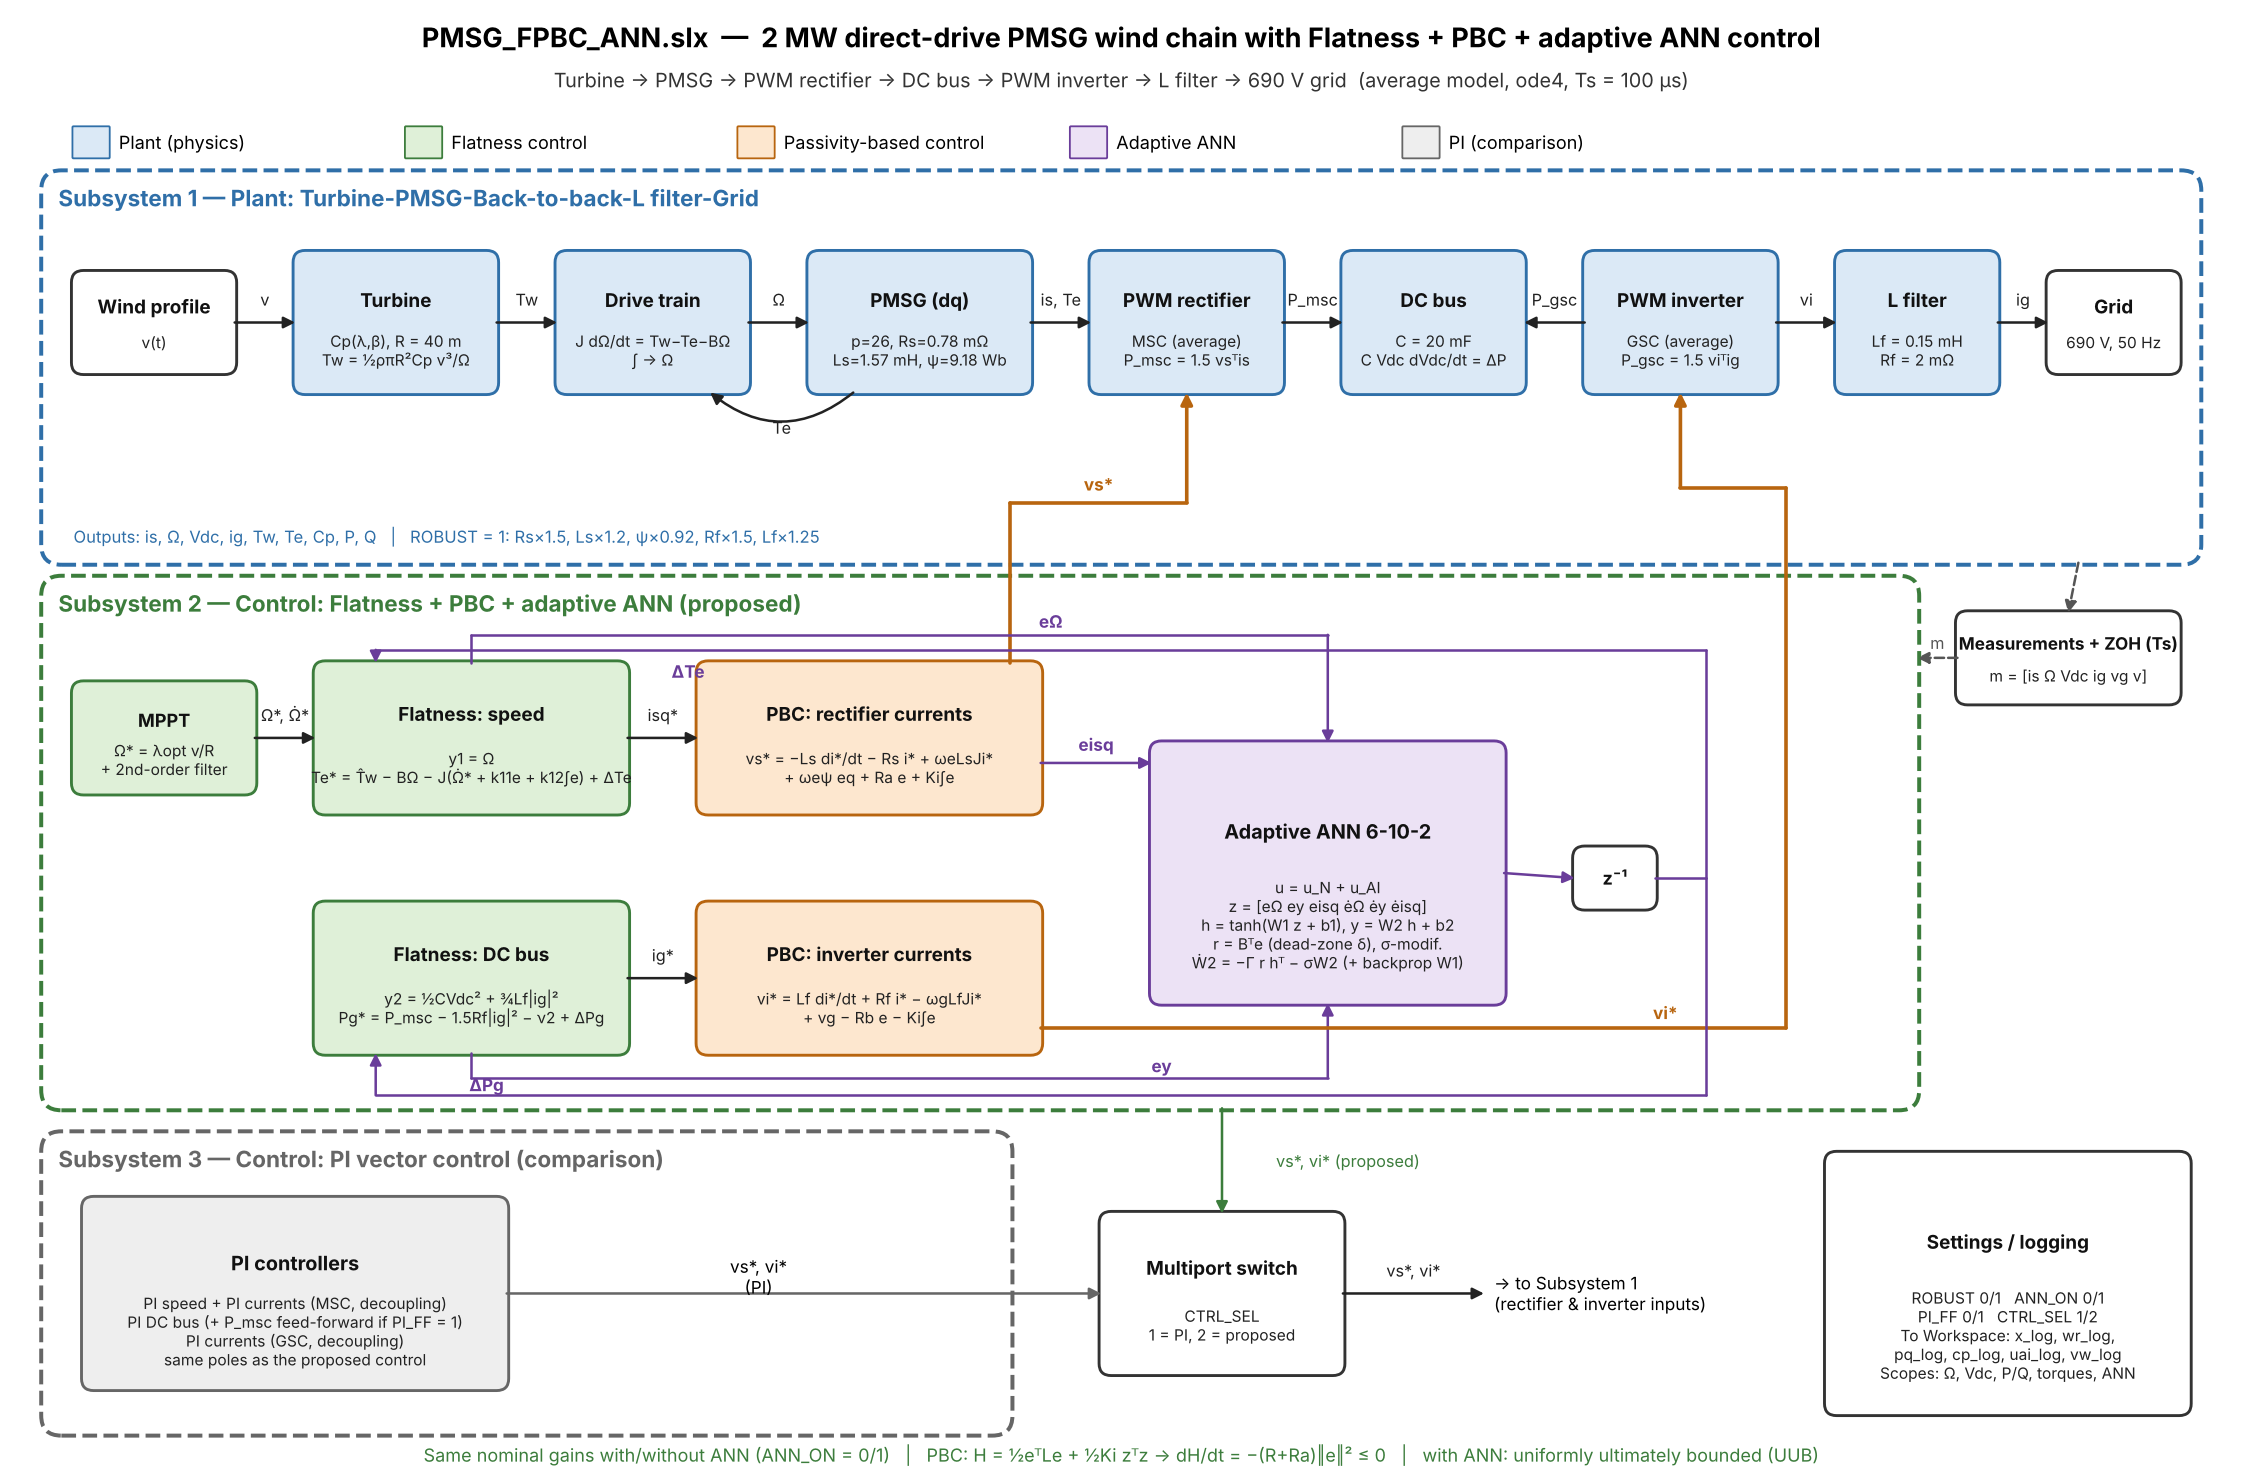
\includegraphics[width=\textwidth]{simulink_diagram.png}
\caption{المخطط الكامل: في الأعلى النظام الفيزيائي، وفي الوسط نظام التحكم.}
\end{figure}

\paragraph{لماذا نحتاج إلى تحكّم (\fr{commande})؟} لثلاثة أسباب:
\begin{enumerate}
\item \textbf{استخراج أكبر طاقة ممكنة}: لكل سرعة ريح توجد سرعة دوران مثلى. يجب أن نجعل التوربينة
تدور بها دائماً (هذا اسمه \fr{MPPT}).
\item \textbf{إبقاء جهد الحافلة المستمرة ثابتاً} (\fr{1200 V}): إذا ارتفع كثيراً تحترق المكثّفات،
وإذا انخفض لا يستطيع المموّج إنتاج جهد الشبكة.
\item \textbf{إرسال طاقة نظيفة إلى الشبكة}: تيار جيبي، و\fr{$Q=0$} (معامل قدرة يساوي 1).
\end{enumerate}

% =====================================================================
\section{النمذجة خطوة بخطوة}
% =====================================================================

\subsection{ما هي النمذجة (\fr{modélisation})؟}
\begin{fikra}
\Fikra
النمذجة هي كتابة \textbf{معادلات} تصف كيف يتغيّر كل متغيّر في النظام مع الزمن.
أغلب معادلاتنا من الشكل:
\[
\frac{d(\text{شيء})}{dt} = \text{ما يدخل} - \text{ما يخرج}.
\]
\textbf{مثال خزّان الماء:} إذا كان الماء الداخل \fr{10 L/s} والخارج \fr{7 L/s}، فإن كمية الماء في الخزّان
تزيد بـ \fr{3 L} كل ثانية. هذا كل شيء! كل معادلات النظام مبنية على هذه الفكرة: «التغيّر = الداخل $-$ الخارج».
\end{fikra}

الرمز $\frac{dx}{dt}$ (أو $\dot x$) يعني «سرعة تغيّر $x$». إذا كانت موجبة، فإن $x$ يزيد؛ وإذا كانت سالبة،
فإنه ينقص؛ وإذا كانت صفراً، فإنه ثابت (نقول إن النظام في «النظام الدائم» \fr{régime permanent}).

\subsection{الريح}
نستعمل نفس معادلة الريح المستعملة في مقالنا في مجلة \fr{Mathematics} (المعادلة 80):
\begin{equation}
v(t) = V_{mean} + \sum_{k=1}^{3} A_k \sin(2\pi f_k t) + v_{turb}(t)
\end{equation}
\begin{itemize}
\item $V_{mean}=8\ \mathrm{m/s}$: السرعة المتوسطة للريح.
\item $\sum A_k\sin(2\pi f_k t)$: ثلاث «موجات» بطيئة تجعل الريح تزيد وتنقص.
القيم: $A=[1{,}5;\ 0{,}2;\ 0{,}3]\ \mathrm{m/s}$ و $f=[0{,}03;\ 0{,}16;\ 0{,}17]\ \mathrm{Hz}$.
\item $v_{turb}(t)$: اضطراب صغير عشوائي (حوالي $\pm 0{,}02\ \mathrm{m/s}$) يمثّل الدوّامات.
\end{itemize}
النتيجة: الريح تبدأ من $8$، تصل إلى $9$ عند $t=2\ \mathrm{s}$، تنزل إلى $8{,}6$، ثم تصعد إلى $10\ \mathrm{m/s}$
عند $t=7{,}7\ \mathrm{s}$.

\subsection{التوربينة: من الريح إلى العزم}

\paragraph{الخطوة 1: كم من الطاقة في الريح؟}
الريح كتلة هواء تتحرّك، فلها طاقة حركية. القدرة التي تمرّ عبر الدائرة التي تمسحها الشفرات (مساحتها
$\pi R^2$) هي:
\begin{equation}
P_{\text{ريح}} = \tfrac12\,\rho\,\pi R^2\, v^3
\end{equation}
حيث $\rho=1{,}225\ \mathrm{kg/m^3}$ كثافة الهواء و $R=40\ \mathrm{m}$ طول الشفرة.
لاحظ: القدرة تتناسب مع $v^3$. إذا تضاعفت الريح، تتضاعف القدرة \textbf{8 مرات}!

\paragraph{الخطوة 2: كم تأخذ التوربينة من هذه الطاقة؟}
التوربينة لا تستطيع أخذ كل الطاقة (وإلا توقّف الهواء خلفها). الجزء المأخوذ هو $C_p$
(معامل القدرة، \fr{coefficient de puissance}):
\begin{equation}
P_w = C_p(\lambda,\beta)\cdot \tfrac12\,\rho\,\pi R^2\, v^3
\end{equation}
نظرياً، لا يمكن أن يتجاوز $C_p$ القيمة $0{,}593$ (حدّ \fr{Betz}). في توربينتنا، القيمة القصوى هي $0{,}48$.

\paragraph{الخطوة 3: ممّا يعتمد $C_p$؟}
يعتمد على \textbf{نسبة السرعة الطرفية} (\fr{vitesse spécifique}):
\begin{equation}
\lambda = \frac{\Omega R}{v} = \frac{\text{سرعة طرف الشفرة}}{\text{سرعة الريح}}
\end{equation}
وعلى زاوية الشفرات $\beta$ (نأخذها $0$ لأن الريح أقل من الاسمية). الصيغة المستعملة (نموذج \fr{Heier}):
\begin{equation}
C_p = 0{,}5176\left(\frac{116}{\lambda_i}-0{,}4\beta-5\right)e^{-21/\lambda_i}+0{,}0068\,\lambda,\qquad
\frac{1}{\lambda_i}=\frac{1}{\lambda+0{,}08\beta}-\frac{0{,}035}{\beta^3+1}
\end{equation}
لا تحتاج إلى حفظها: المهم هو شكلها (الشكل \ref{fig:cp}). هناك قيمة واحدة $\lambda_{opt}=8{,}1$ تعطي أكبر $C_p$.

\begin{figure}[h]
\centering
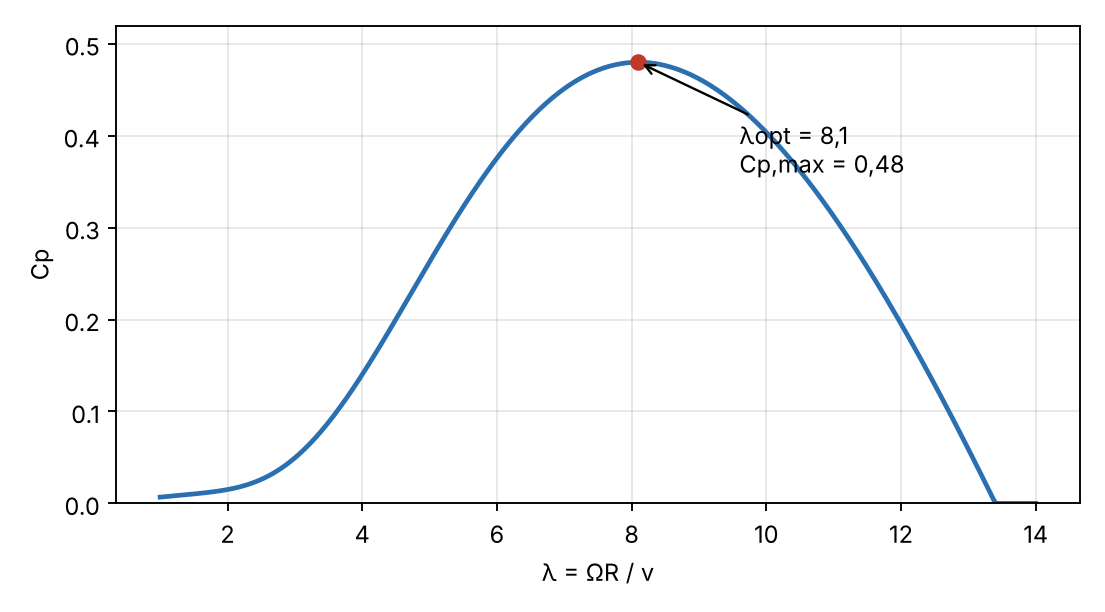
\includegraphics[width=0.62\textwidth]{cp_lambda.png}
\caption{معامل القدرة $C_p$ بدلالة $\lambda$: يوجد قمّة واحدة عند $\lambda_{opt}=8{,}1$.}
\label{fig:cp}
\end{figure}

\paragraph{الخطوة 4: العزم الهوائي.}
القدرة = العزم $\times$ السرعة الزاوية، إذن:
\begin{equation}
T_w = \frac{P_w}{\Omega}
\end{equation}

\begin{mithal}
\Mithal
ريح $v=8\ \mathrm{m/s}$. مساحة الدوران: $\pi\times 40^2 = 5027\ \mathrm{m^2}$.
\begin{itemize}
\item القدرة في الريح: $\tfrac12\times 1{,}225\times 5027\times 8^3 = 1{,}58\ \mathrm{MW}$.
\item السرعة المثلى: $\Omega = \lambda_{opt}\,v/R = 8{,}1\times 8/40 = 1{,}62\ \mathrm{rad/s}$ (حوالي $15{,}5$ دورة في الدقيقة).
\item القدرة المأخوذة: $0{,}48\times 1{,}58 = 0{,}76\ \mathrm{MW}$.
\item العزم: $T_w = 0{,}76\cdot 10^6/1{,}62 = 467\ \mathrm{kN\cdot m}$.
\end{itemize}
وعند الريح الاسمية ($\approx 11\ \mathrm{m/s}$): $\Omega = 2{,}23\ \mathrm{rad/s}$ و $P\approx 2\ \mathrm{MW}$، وهي فعلاً قدرة
التوربينة. هذا يؤكّد أن أرقام الأستاذ متناسقة.
\end{mithal}

\subsection{العمود (\fr{arbre}): من العزم إلى السرعة}
\begin{fikra}
\Fikra
هذا هو قانون نيوتن للدوران. الريح تدفع (عزم $T_w$)، والمولّد «يكبح» (عزم $T_e$)، والاحتكاك يكبح قليلاً.
إذا كان الدفع أكبر من الكبح، تتسارع التوربينة؛ وإذا كان أصغر، تتباطأ.
\end{fikra}
\begin{equation}
J\,\frac{d\Omega}{dt} = T_w - T_e - B\,\Omega
\end{equation}
\begin{itemize}
\item $J=2{,}8\cdot10^6\ \mathrm{kg\cdot m^2}$: عطالة الدوران (كلّما كبرت، صعب تغيير السرعة).
\item $T_e$: العزم الكهرومغناطيسي للمولّد. \textbf{هذا هو ما نتحكّم فيه!}
\item $B\Omega$: الاحتكاك ($B=1000$).
\end{itemize}

\begin{mithal}
\Mithal
إذا كان $T_w - T_e = 100\ \mathrm{kN\cdot m}$، فإن $\frac{d\Omega}{dt} = 10^5/(2{,}8\cdot 10^6) = 0{,}036\ \mathrm{rad/s^2}$.
للانتقال من $1{,}62$ إلى $1{,}82\ \mathrm{rad/s}$ (عندما تصير الريح $9\ \mathrm{m/s}$) نحتاج حوالي $5{,}6$ ثوانٍ.
التوربينة ثقيلة جداً، فهي بطيئة.
\end{mithal}

\textbf{الفكرة المهمّة للتحكّم:} لكي نجعل التوربينة تدور بالسرعة المثلى، نتحكّم في $T_e$:
\begin{itemize}
\item إذا كانت أبطأ من اللازم، ننقص $T_e$ (نكبح أقل) فتتسارع؛
\item إذا كانت أسرع من اللازم، نزيد $T_e$ (نكبح أكثر) فتتباطأ.
\end{itemize}

\subsection{المولّد \fr{PMSG}: من الدوران إلى الكهرباء}

\paragraph{الخطوة 1: كيف يولّد الكهرباء؟}
الدوّار (\fr{rotor}) فيه مغانط دائمة. عندما يدور، يتغيّر الحقل المغناطيسي داخل ملفات الساكن
(\fr{stator})، فتظهر فيها قوة محرّكة كهربائية (\fr{f.é.m.}) تتناسب مع السرعة:
$E = \omega_e\,\psi_f$، حيث $\psi_f=9{,}18\ \mathrm{Wb}$ هو تدفّق المغانط.

\paragraph{الخطوة 2: ثلاثة أطوار، ثم تحويل \fr{Park}.}
المولّد ثلاثي الأطوار: له ثلاثة تيارات $i_a, i_b, i_c$ جيبية ومتغيّرة باستمرار. التحكّم في أشياء
تتأرجح صعب. لذلك نستعمل \textbf{تحويل \fr{Park}}: نصف التيارات من وجهة نظر شخص يدور مع الدوّار.
من وجهة نظره، التيارات لا تتأرجح، بل تصبح \textbf{قيمتين ثابتتين} تقريباً:
\begin{itemize}
\item $i_{sd}$ (المحور \fr{d}): على اتجاه المغانط. لا ينتج عزماً.
\item $i_{sq}$ (المحور \fr{q}): عمودي على المغانط. هو الذي ينتج العزم.
\end{itemize}
\begin{fikra}
\Fikra
تحويل \fr{Park} مثل الركوب على دوّامة الملاهي: الأشياء التي تدور معك تبدو لك ثابتة.
هكذا تصبح الكميات المتناوبة كميات «مستمرة»، فيصبح التحكّم فيها سهلاً.
\end{fikra}

\paragraph{الخطوة 3: معادلات الجهد.}
لكل محور، نكتب قانون \fr{Kirchhoff}: «الجهد الناتج داخل الآلة = الجهد الضائع + الجهد الخارج».
\begin{align}
L_s\frac{di_{sd}}{dt} &= \underbrace{-R_s i_{sd}}_{\text{ضياع في المقاومة}}
\;+\;\underbrace{\omega_e L_s i_{sq}}_{\text{تأثير المحور الآخر}}
\;-\;\underbrace{v_{sd}}_{\text{جهد المقوّم}}\\
L_s\frac{di_{sq}}{dt} &= -R_s i_{sq} - \omega_e L_s i_{sd}
\;+\;\underbrace{\omega_e\psi_f}_{\text{القوة المحرّكة }E} \;-\; v_{sq}
\end{align}
\begin{itemize}
\item $R_s=0{,}78\ \mathrm{m\Omega}$: مقاومة الملفات. $L_s=1{,}57\ \mathrm{mH}$: الحثّ (يقاوم تغيّر التيار).
\item $\omega_e = p\,\Omega$: السرعة الكهربائية، و $p=26$ عدد أزواج الأقطاب.
\item $\omega_e L_s i$: حدود «تزاوج» (\fr{couplage}) بين المحورين، سببها أن المرجع يدور.
\item $v_{sd}, v_{sq}$: الجهد الذي يفرضه المقوّم. \textbf{هذا ما نتحكّم فيه} لنتحكّم في التيارات.
\end{itemize}

\paragraph{الخطوة 4: العزم.}
\begin{equation}
T_e = \tfrac32\, p\, \psi_f\, i_{sq}
\end{equation}
العزم يتناسب مع $i_{sq}$ فقط. لذلك نختار $i_{sd}^*=0$ (لا فائدة منه، ويسبّب ضياعاً)، ونتحكّم في
العزم عبر $i_{sq}$.

\begin{mithal}
\Mithal
عند $\Omega=1{,}62\ \mathrm{rad/s}$: $\omega_e = 26\times 1{,}62 = 42{,}1\ \mathrm{rad/s}$، أي تردّد
$6{,}7\ \mathrm{Hz}$ (وليس $50$!). القوة المحرّكة: $E = 9{,}18\times 42{,}1 = 387\ \mathrm{V}$.
لإنتاج $T_e = 467\ \mathrm{kN\cdot m}$ نحتاج $i_{sq} = 467000/(1{,}5\times 26\times 9{,}18) = 1304\ \mathrm{A}$.
\end{mithal}

\paragraph{الخطوة 5: الكتابة المصفوفية وخاصية مهمّة جداً.}
نجمع المعادلتين: $\bv{i}_s=[i_{sd};\ i_{sq}]$، $\bv{v}_s=[v_{sd};\ v_{sq}]$، و
$\mathbf{J}=\begin{bmatrix}0&1\\-1&0\end{bmatrix}$:
\begin{equation}
L_s\,\dot{\bv{i}}_s = -R_s\,\bv{i}_s + \omega_e L_s\,\mathbf{J}\,\bv{i}_s + \omega_e\psi_f\,\bv{e}_q - \bv{v}_s
\end{equation}
المصفوفة $\mathbf{J}$ «مضادّة للتناظر» (\fr{antisymétrique}): $\bv{i}^T\mathbf{J}\,\bv{i} = i_d i_q - i_q i_d = 0$.
\begin{fikra}
\Fikra
معنى ذلك أن حدّ التزاوج $\omega_e L_s\mathbf{J}\bv{i}_s$ \textbf{لا ينتج ولا يستهلك طاقة}، بل ينقلها فقط
بين المحورين (مثل قوة تدير الشيء دون أن تسرّعه). نسمّيه «بدون عمل» (\fr{sans travail}).
هذه الخاصية هي أساس التحكّم بالسلبية لاحقاً.
\end{fikra}

\subsection{المحوّلات \fr{MLI}: المقوّم والمموّج}
\paragraph{ماذا تفعل الـ \fr{MLI} (\fr{PWM})؟}
المحوّل مكوّن من مفاتيح إلكترونية (\fr{IGBT}) تفتح وتغلق بسرعة كبيرة ($2160$ مرة في الثانية).
بتغيير مدّة الفتح (\fr{rapport cyclique})، نصنع جهداً «متوسطاً» بالقيمة التي نريد.
\begin{fikra}
\Fikra
مثل مصباح تشعله وتطفئه بسرعة كبيرة: إذا كان مشتعلاً نصف الوقت، ترى نصف الضوء.
\end{fikra}

\paragraph{النموذج المتوسط (\fr{modèle moyen}).}
لا نهتمّ بكل فتح وإغلاق، بل بالقيمة المتوسطة فقط. نعتبر إذن أن المحوّل يعطي مباشرة الجهد الذي
نطلبه، بشرط ألّا يتجاوز حداً أقصى:
\begin{equation}
\|\bv{v}\| \le \frac{V_{dc}}{\sqrt3} = \frac{1200}{1{,}732} = 693\ \mathrm{V}
\end{equation}
والمحوّل لا يضيّع طاقة (نفترض ذلك)، إذن القدرة الداخلة = القدرة الخارجة:
\begin{equation}
P_{msc} = \tfrac32\,(v_{sd}i_{sd}+v_{sq}i_{sq}),\qquad P_{gsc} = \tfrac32\,(v_{id}i_{gd}+v_{iq}i_{gq})
\end{equation}

\subsection{الحافلة المستمرة (\fr{bus DC}): خزّان الطاقة}
المكثّف ($C=20\ \mathrm{mF}$) مثل خزّان ماء: المقوّم يملؤه بـ $P_{msc}$، والمموّج يفرغه بـ $P_{gsc}$.
الطاقة المخزّنة $W = \tfrac12 C V_{dc}^2$، و«التغيّر = الداخل $-$ الخارج»:
\begin{equation}
\frac{dW}{dt} = P_{msc} - P_{gsc}\qquad\Longleftrightarrow\qquad C\,V_{dc}\frac{dV_{dc}}{dt}=P_{msc}-P_{gsc}
\end{equation}
\begin{mithal}
\Mithal
عند $1200\ \mathrm{V}$: $W = 0{,}5\times 0{,}02\times 1200^2 = 14{,}4\ \mathrm{kJ}$ فقط.
إذا دخل $100\ \mathrm{kW}$ أكثر مما خرج، يتغيّر المخزون كله في $14{,}4/100 = 0{,}14\ \mathrm{s}$!
لذلك يجب أن يكون التحكّم في هذه الحافلة \textbf{سريعاً جداً}.
\end{mithal}

\subsection{المرشّح \fr{L} والشبكة}
المرشّح ملف ($L_f=0{,}15\ \mathrm{mH}$، $R_f=2\ \mathrm{m\Omega}$) بين المموّج والشبكة. يعمل مثل
\fr{PMSG} تماماً، لكن «القوة المحرّكة» هنا هي جهد الشبكة $\bv{v}_g$:
\begin{equation}
L_f\,\dot{\bv{i}}_g = -R_f\,\bv{i}_g + \omega_g L_f\,\mathbf{J}\,\bv{i}_g + \bv{v}_i - \bv{v}_g
\end{equation}
نختار مرجع \fr{Park} موجّهاً على جهد الشبكة (\fr{PLL}): $v_{gd}=563\ \mathrm{V}$ و $v_{gq}=0$. عندئذ:
\begin{equation}
P = \tfrac32\,v_{gd}\,i_{gd},\qquad Q = -\tfrac32\,v_{gd}\,i_{gq}
\end{equation}
إذن $i_{gd}$ يتحكّم في القدرة الفعّالة $P$، و $i_{gq}$ يتحكّم في القدرة الردّية $Q$ (نريد $Q=0$، إذن $i_{gq}^*=0$).

\subsection{النموذج الكامل: 6 متغيّرات}
\begin{khulasa}
\Khulasa
النظام كله يوصف بـ 6 متغيّرات (المتغيّرات الحالية \fr{variables d'état})، لكل واحد معادلته:
\begin{center}
\begin{tabular}{lll}
\toprule
المتغيّر & معناه & المعادلة التي تحكمه\\
\midrule
$i_{sd}, i_{sq}$ & تيارات المولّد & معادلات \fr{PMSG}\\
$\Omega$ & سرعة الدوران & قانون نيوتن للعمود\\
$V_{dc}$ & جهد الحافلة & توازن الطاقة في المكثّف\\
$i_{gd}, i_{gq}$ & تيارات الشبكة & معادلات المرشّح\\
\bottomrule
\end{tabular}
\end{center}
\textbf{ما نتحكّم فيه} (4 مداخل): $v_{sd}, v_{sq}$ (المقوّم) و $v_{id}, v_{iq}$ (المموّج).\\
\textbf{ما لا نتحكّم فيه} (اضطرابات): الريح $v$ وجهد الشبكة $v_g$.
\end{khulasa}

\subsection{الأرقام (\fr{paramètres})}
\begin{center}
\begin{tabular}{llll}
\toprule
العنصر & الرمز & القيمة & المصدر\\
\midrule
القدرة الاسمية & $P_n$ & $2\ \mathrm{MW}$ & الأستاذ\\
طول الشفرة & $R$ & $40\ \mathrm{m}$ & الأستاذ\\
السرعة الاسمية & $\Omega_n$ & $2{,}23\ \mathrm{rad/s}$ & الأستاذ\\
العزم الاسمي & $T_n$ & $0{,}9\ \mathrm{MN\cdot m}$ & الأستاذ\\
أزواج الأقطاب & $p$ & $26$ & مقال \fr{Hasan \& Shatil}\\
مقاومة الساكن & $R_s$ & $0{,}78\ \mathrm{m\Omega}$ & نفس المقال\\
الحثّ & $L_s$ & $1{,}57\ \mathrm{mH}$ & نفس المقال\\
تدفّق المغانط & $\psi_f$ & $9{,}18\ \mathrm{Wb}$ & نفس المقال\\
المكثّف & $C$ & $20\ \mathrm{mF}$ & نفس المقال\\
جهد الحافلة & $V_{dc}^*$ & $1200\ \mathrm{V}$ & نفس المقال\\
حثّ المرشّح & $L_f$ & $0{,}15\ \mathrm{mH}$ & نفس المقال\\
العطالة & $J$ & $2{,}8\cdot10^6\ \mathrm{kg\cdot m^2}$ & فرضية\\
الشبكة & & $690\ \mathrm{V}$، $50\ \mathrm{Hz}$ & نفس المقال\\
\bottomrule
\end{tabular}
\end{center}

% =====================================================================
\section{التحكّم خطوة بخطوة}
% =====================================================================

\subsection{ما هو التحكّم؟}
\begin{fikra}
\Fikra
مثال: تريد أن تسير سيارتك بـ $80\ \mathrm{km/h}$ (هذا هو \textbf{المرجع} \fr{référence}). تنظر إلى العدّاد
(\textbf{القياس} \fr{mesure})، وتحسب الفرق (\textbf{الخطأ} \fr{erreur}): إذا كنت بـ $70$، فالخطأ $+10$،
فتضغط على البنزين (\textbf{الأمر} \fr{commande}). هذه هي «الحلقة المغلقة» (\fr{boucle fermée}).
كل نظام تحكّم يجيب عن سؤال واحد: \textbf{بأيّ قدر نضغط، بدلالة الخطأ؟}
\end{fikra}

في كل ما يلي: $x^*$ هو المرجع (القيمة المطلوبة)، و $e = x^* - x$ أو $e = x - x^*$ هو الخطأ.

\subsection{لماذا حلقات متداخلة (\fr{cascade})؟}
لدينا أشياء بطيئة (السرعة: ثوانٍ) وأشياء سريعة جداً (التيارات: أجزاء من الألف من الثانية).
لذلك نضع حلقتين:
\begin{itemize}
\item \textbf{حلقة خارجية بطيئة}: تقرّر «ماذا نريد» (العزم المطلوب، أو القدرة المطلوبة).
\item \textbf{حلقة داخلية سريعة}: تنفّذ ذلك بالتحكّم في التيارات.
\end{itemize}
\begin{figure}[h]
\centering
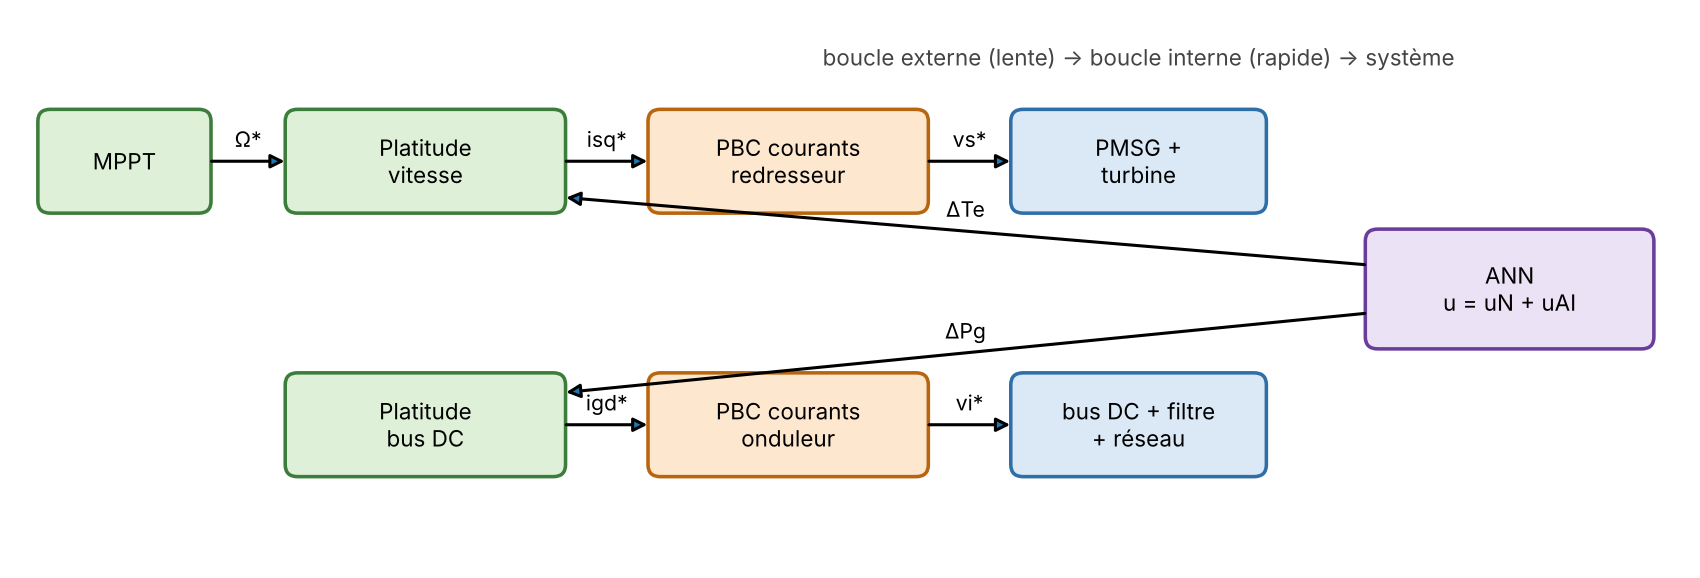
\includegraphics[width=\textwidth]{cascade.png}
\caption{بنية التحكّم: في الأعلى جانب الآلة، وفي الأسفل جانب الشبكة، وعلى اليمين الشبكة العصبونية التي
تضيف تصحيحاً.}
\end{figure}

\subsection{المرحلة 1: الـ \fr{MPPT} (أين نريد أن نكون؟)}
\begin{figure}[h]
\centering
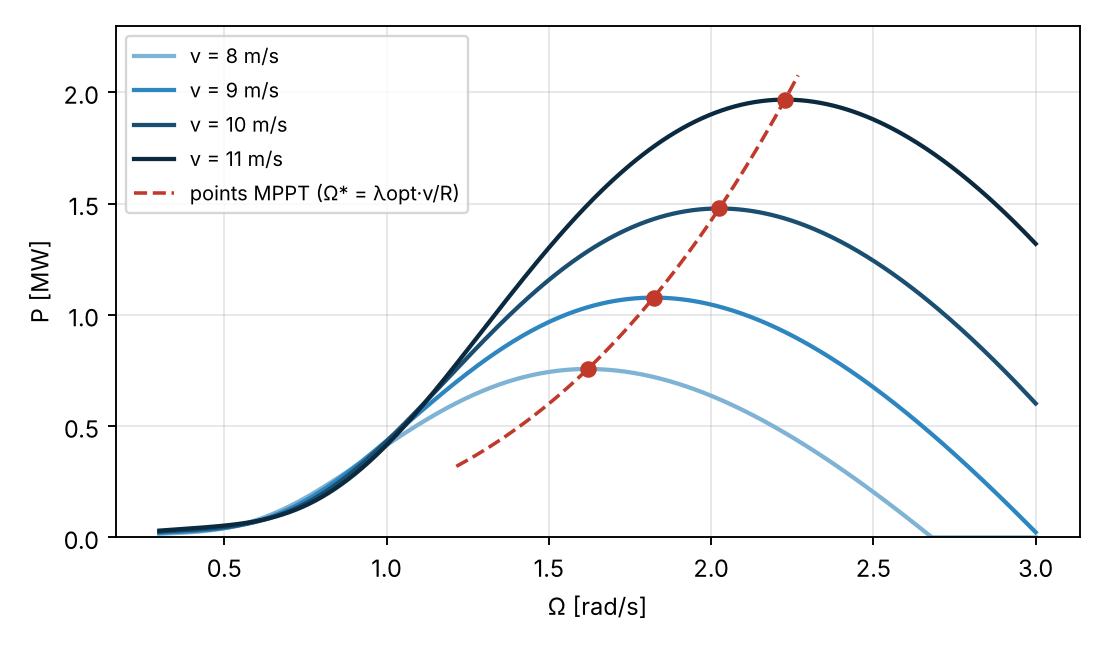
\includegraphics[width=0.62\textwidth]{mppt.png}
\caption{القدرة بدلالة السرعة لعدّة سرعات ريح. النقاط الحمراء هي القمم: هناك نريد أن نكون.}
\end{figure}
لكل ريح، القدرة القصوى تكون عند $\lambda=\lambda_{opt}$، أي:
\begin{equation}
\Omega^* = \frac{\lambda_{opt}\, v}{R}
\end{equation}
هذه هي «السرعة المرجعية». نمرّرها في مرشّح يجعلها ناعمة، ويعطي أيضاً مشتقّتها $\dot\Omega^*$
(سنحتاجها).

\subsection{تذكير بالمنظّم \fr{PI} (لفهم ما يلي)}
أبسط تحكّم هو المنظّم \fr{PI}: $u = K_p\, e + K_i\int e\,dt$.
\begin{itemize}
\item الجزء $K_p\,e$ (\textbf{تناسبي}): كلّما كبر الخطأ، كبر التصحيح.
\item الجزء $K_i\int e$ (\textbf{تكاملي}): يتذكّر الأخطاء الماضية، فيزيل الخطأ الصغير الذي يبقى في النهاية.
\end{itemize}
سنجد هذين الجزأين في كل قوانيننا (المعاملات $k_{11}, k_{12}$ إلخ). الفرق أن قوانيننا تستعمل أيضاً
\textbf{النموذج الفيزيائي}، فتكون أدقّ.

\subsection{المرحلة 2: التحكّم بالتسطيح (\fr{platitude})}

\paragraph{الفكرة بكلمات بسيطة.}
\begin{fikra}
\Fikra
بدل أن ننتظر الخطأ لكي نصحّح (مثل \fr{PI})، نستعمل المعادلة الفيزيائية \textbf{بالمقلوب}:
«أريد أن تتحرّك السرعة هكذا؛ إذن ما هو العزم الذي يجب أن أطبّقه؟». المعادلة تعطينا الجواب مباشرة.
ثم نضيف تصحيحاً صغيراً (مثل \fr{PI}) لما لا يعرفه النموذج.
نقول إن النظام «مسطّح» (\fr{plat}) إذا كان يمكن حساب كل شيء (الحالات والأوامر) من «مخرج» واحد
ومشتقّاته. هذا المخرج اسمه «المخرج المسطّح» (\fr{sortie plate}).
\end{fikra}

\paragraph{حلقة السرعة، خطوة بخطوة.}
\begin{enumerate}
\item نبدأ من معادلة العمود: $J\dot\Omega = T_w - T_e - B\Omega$.
\item نقلبها لنحسب العزم: $T_e = T_w - B\Omega - J\dot\Omega$.
إذن إذا عرفنا $\Omega$ و $\dot\Omega$، نعرف $T_e$. المخرج المسطّح هو $y_1=\Omega$.
\item ماذا نريد لـ $\dot\Omega$؟ نريد أن تتبع $\Omega$ المرجع $\Omega^*$. نختار:
\[
\nu_1 = \underbrace{\dot\Omega^*}_{\text{اتبع المرجع}} + \underbrace{k_{11}\,e_\Omega}_{\text{صحّح الخطأ}} + \underbrace{k_{12}\!\int\! e_\Omega}_{\text{أزل الخطأ الباقي}},
\qquad e_\Omega = \Omega^* - \Omega
\]
\item نعوّض $\dot\Omega$ بـ $\nu_1$، ونعوّض $T_w$ (لا نقيسه) بقيمته المحسوبة $\hat T_w$ من معادلة $C_p$ والريح المقاسة:
\begin{equation}
\boxed{T_e^* = \hat T_w - B\,\Omega - J\,\nu_1 + \Delta T_e}
\end{equation}
($\Delta T_e$ هو تصحيح الشبكة العصبونية، سنشرحه لاحقاً.)
\item نحوّل العزم إلى تيار: $i_{sq}^* = T_e^*/(1{,}5\,p\,\psi_f)$ و $i_{sd}^*=0$.
\end{enumerate}
\textbf{لماذا يعمل؟} إذا كان $\hat T_w = T_w$ تماماً، نعوّض في معادلة العمود فنجد:
\[
\dot e_\Omega + k_{11}\,e_\Omega + k_{12}\!\int\! e_\Omega = 0 .
\]
هذه معادلة خطأ «يموت» تلقائياً (مثل نابض مع ممتصّ صدمات). نختار $k_{11}=2\zeta\omega_n=3{,}6$ و
$k_{12}=\omega_n^2=4$ (مع $\omega_n = 2\ \mathrm{rad/s}$ و $\zeta=0{,}9$)، أي أن الخطأ يختفي في حوالي ثانيتين
بدون تذبذب كبير.

\paragraph{حلقة الحافلة المستمرة، خطوة بخطوة.}
\begin{enumerate}
\item المخرج المسطّح هنا هو \textbf{الطاقة المخزّنة} (في المكثّف وفي ملفات المرشّح):
$y_2 = \tfrac12 C V_{dc}^2 + \tfrac34 L_f\|\bv{i}_g\|^2$.
\item لماذا الطاقة وليس الجهد؟ لأن معادلة الطاقة \textbf{خطّية وبسيطة}: «التغيّر = الداخل $-$ الخارج»:
\[
\dot y_2 = P_{msc} - \underbrace{\tfrac32 v_{gd} i_{gd}}_{P_g\ \text{(إلى الشبكة)}} - \underbrace{\tfrac32 R_f\|\bv{i}_g\|^2}_{\text{ضياع المرشّح}}
\]
\item نقلبها: لكي يكون $\dot y_2 = -\nu_2$، يجب أن نرسل للشبكة:
\begin{equation}
\boxed{P_g^* = P_{msc} - \tfrac32 R_f\|\bv{i}_g\|^2 - \nu_2 + \Delta P_g},\qquad
\nu_2 = k_{21}\,e_y + k_{22}\!\int\! e_y,\quad e_y = y_2^*-y_2
\end{equation}
\item بالكلمات: «أرسل للشبكة كل ما يأتي من المولّد ($P_{msc}$)، ناقص الضياع، وصحّح قليلاً إذا كانت
الطاقة المخزّنة بعيدة عن المرجع».
\item نحوّل القدرة إلى تيار: $i_{gd}^* = 2P_g^*/(3 v_{gd})$ و $i_{gq}^* = 0$.
\end{enumerate}
\textbf{لماذا هذا جيّد؟} لأن القانون \textbf{يتوقّع} (\fr{anticipe}): بمجرّد أن تتغيّر $P_{msc}$، يتغيّر
$P_g^*$ فوراً، قبل أن يتغيّر الجهد. لذلك يبقى $V_{dc}$ ثابتاً تقريباً ($\pm 0{,}4\ \mathrm{V}$).

\subsection{المرحلة 3: التحكّم بالسلبية (\fr{passivité}، \fr{PBC}) في التيارات}

\paragraph{الفكرة بكلمات بسيطة.}
\begin{fikra}
\Fikra
النظام «السلبي» (\fr{passif}) هو نظام لا يصنع طاقة من العدم: طاقته المخزّنة لا يمكن أن تزيد إلا إذا
أعطيناه طاقة من الخارج. مثل كرة في وعاء: إذا تركتها، تتدحرج ثم تتوقّف في القاع بسبب الاحتكاك.\\
التحكّم بالسلبية يقول: \textbf{اجعل «طاقة الخطأ» تتصرّف مثل هذه الكرة.} نكتب طاقة للخطأ، ونصمّم
الأمر بحيث تنقص هذه الطاقة دائماً. عندئذ يذهب الخطأ إلى الصفر حتماً.
\end{fikra}

\paragraph{خطوة بخطوة (للمقوّم).}
\begin{enumerate}
\item نعرّف الخطأ: $\bv{e}_s = \bv{i}_s - \bv{i}_s^*$.
\item نريد أن يكون للخطأ نفس شكل معادلة \fr{PMSG}، مع \textbf{احتكاك إضافي} $R_a$ (نسمّيه «حقن التخميد»
\fr{injection d'amortissement}، مثل ممتصّ الصدمات في السيارة)، ومع جزء تكاملي $K_i$:
\[
L_s\dot{\bv{e}}_s = -(R_s+R_a)\,\bv{e}_s + \omega_e L_s\,\mathbf{J}\,\bv{e}_s - K_i\!\int\!\bv{e}_s
\]
\item لكي نحصل على هذا، نحسب الجهد الذي يجب أن يطبّقه المقوّم (نعوّض في معادلة \fr{PMSG} ونحلّ):
\begin{equation}
\boxed{\bv{v}_s^* = -L_s\dot{\bv{i}}_s^* - R_s\bv{i}_s^* + \omega_e L_s\mathbf{J}\,\bv{i}_s^* + \omega_e\psi_f\,\bv{e}_q + R_a\,\bv{e}_s + K_i\!\int\!\bv{e}_s}
\end{equation}
حدّاً بحدّ:
\begin{itemize}
\item $-L_s\dot{\bv{i}}_s^* - R_s\bv{i}_s^*$: الجهد اللازم «نظرياً» لكي يتبع التيار مرجعه.
\item $\omega_e L_s\mathbf{J}\bv{i}_s^*$: نترك التزاوج كما هو (لأنه بدون عمل) لكن على المرجع.
\item $\omega_e\psi_f\bv{e}_q$: نعوّض القوة المحرّكة للمولّد.
\item $R_a\bv{e}_s$: الاحتكاك الإضافي الذي يقتل الخطأ.
\item $K_i\int\bv{e}_s$: يزيل الخطأ الصغير الباقي (إذا كانت البارامترات غير دقيقة).
\end{itemize}
\end{enumerate}

\paragraph{لماذا هذا مستقرّ؟ (البرهان بالكلمات)}
نأخذ «طاقة الخطأ»:
\[
H = \underbrace{\tfrac12 L_s\|\bv{e}_s\|^2}_{\text{طاقة مغناطيسية للخطأ}} + \underbrace{\tfrac12 K_i\|\textstyle\int\bv{e}_s\|^2}_{\text{طاقة الجزء التكاملي}}
\]
نحسب كيف تتغيّر، فنجد:
\[
\frac{dH}{dt} = -(R_s+R_a)\,\|\bv{e}_s\|^2 \;+\; \underbrace{\omega_e L_s\,\bv{e}_s^T\mathbf{J}\,\bv{e}_s}_{=0\ \text{(بدون عمل!)}} \;=\; -(R_s+R_a)\,\|\bv{e}_s\|^2 \le 0 .
\]
\begin{khulasa}
\Khulasa
طاقة الخطأ \textbf{لا تزيد أبداً}، وتنقص ما دام هناك خطأ. إذن الخطأ يذهب إلى الصفر.
هنا استعملنا خاصية «بدون عمل» للمصفوفة $\mathbf{J}$: حدّ التزاوج اختفى من الحساب.
هذا هو جوهر التحكّم بالسلبية: \textbf{نحترم بنية الطاقة في النظام بدل أن نحاربها}.
\end{khulasa}

نفس الشيء للمموّج والمرشّح:
\begin{equation}
\boxed{\bv{v}_i^* = L_f\dot{\bv{i}}_g^* + R_f\bv{i}_g^* - \omega_g L_f\mathbf{J}\,\bv{i}_g^* + \bv{v}_g - R_b\,\bv{e}_g - K_{ig}\!\int\!\bv{e}_g}
\end{equation}

\paragraph{الأرقام.} نختار ثابت زمن $\tau_i = 2\ \mathrm{ms}$ (التيارات سريعة جداً):
$R_a = L_s/\tau_i = 0{,}785\ \Omega$ و $R_b = L_f/\tau_i = 0{,}075\ \Omega$.

\subsection{ما هي «دالة ليابونوف» (\fr{Lyapunov})؟}
\begin{fikra}
\Fikra
دالة ليابونوف هي «طاقة» نخترعها للخطأ: تكون موجبة دائماً، وتساوي صفراً فقط عندما يكون الخطأ صفراً.
إذا أثبتنا أنها \textbf{تنقص دائماً} مع الزمن، فالخطأ مجبر على الذهاب إلى الصفر، مثل كرة تنزل في
وعاء حتى القاع. الدالة $H$ التي استعملناها أعلاه هي دالة ليابونوف.
\end{fikra}

% =====================================================================
\section{الشبكة العصبونية (\fr{ANN}) خطوة بخطوة}
% =====================================================================

\subsection{لماذا نحتاجها؟}
قانون التسطيح يستعمل $\hat T_w$ المحسوب من معادلة $C_p$. لكن في الواقع، معادلة $C_p$ \textbf{ليست دقيقة
أبداً} (الشفرات تتّسخ، كثافة الهواء تتغيّر...). في اختبار المتانة جعلنا $\hat T_w$ أصغر بـ $10\%$ من
الحقيقة. النتيجة: يبقى خطأ صغير في السرعة لا يُزال بسرعة.
\begin{fikra}
\Fikra
الشبكة العصبونية «تتعلّم» هذا الخطأ أثناء التشغيل وتصحّحه. هي \textbf{لا تعوّض} التحكّم الأساسي،
بل \textbf{تضيف} تصحيحاً صغيراً:
\[
u = \underbrace{u_N}_{\text{التحكّم الأساسي}} + \underbrace{u_{AI}}_{\text{تصحيح الشبكة}},
\qquad u_{AI} = [\Delta T_e;\ \Delta P_g]
\]
ولا تغيّر معاملات التحكّم الأساسي ($k_{11}$، $R_a$ إلخ). هذه نفس طريقة مقالنا في \fr{Mathematics}.
\end{fikra}

\subsection{العصبون الواحد (\fr{neurone})}
العصبون عملية حسابية بسيطة جداً:
\begin{enumerate}
\item يأخذ عدّة مداخل $z_1, z_2, \dots$
\item يضرب كل مدخل في «وزن» (\fr{poids}) $w_1, w_2, \dots$ ويجمعها، ويضيف «انحيازاً» (\fr{biais}) $b$:
$\ a = w_1 z_1 + w_2 z_2 + \dots + b$
\item يمرّر النتيجة في «دالة تنشيط» (\fr{fonction d'activation}). نستعمل $\tanh$، وهي تشبه حرف \fr{S}:
تعطي قيمة بين $-1$ و $+1$.
\end{enumerate}
\begin{mithal}
\Mithal
مدخلان $z=[0{,}5;\ -0{,}2]$، وأوزان $w=[0{,}8;\ 0{,}3]$، و $b=0{,}1$:\\
$a = 0{,}8\times 0{,}5 + 0{,}3\times(-0{,}2) + 0{,}1 = 0{,}44$، والمخرج $h = \tanh(0{,}44) = 0{,}41$.
\end{mithal}
\textbf{الأوزان هي «ذاكرة» الشبكة.} التعلّم معناه تعديل الأوزان.

\subsection{الشبكة 6-10-2}
\begin{figure}[h]
\centering
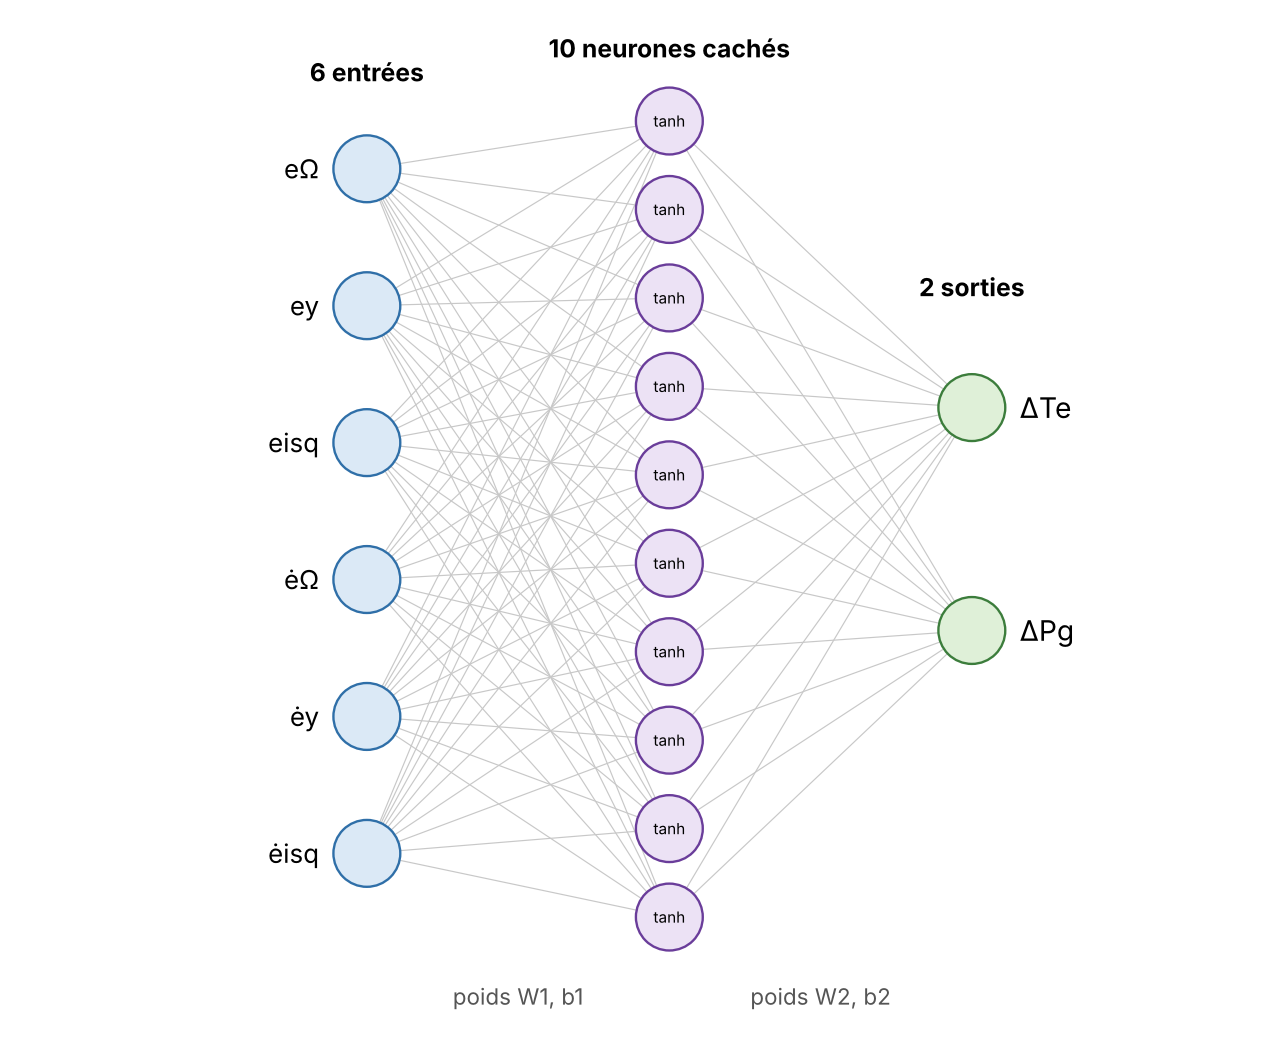
\includegraphics[width=0.6\textwidth]{ann.png}
\caption{الشبكة العصبونية: 6 مداخل، 10 عصبونات مخفية، مخرجان.}
\end{figure}
\begin{itemize}
\item \textbf{6 مداخل}: الأخطاء الثلاثة ومشتقّاتها:
$e_\Omega$ (خطأ السرعة)، $e_y$ (خطأ طاقة الحافلة)، $e_{isq}$ (خطأ التيار)، و $\dot e_\Omega, \dot e_y, \dot e_{isq}$.
نقسمها على قيم مرجعية (\fr{normalisation}) لكي تكون كلها من نفس الحجم (حول 1).
\item \textbf{10 عصبونات مخفية} (\fr{couche cachée}): كل واحد يحسب $h_j = \tanh(\sum_i W_{1,ji} z_i + b_{1,j})$.
بالمصفوفات: $\bv{h} = \tanh(W_1\bv{z} + \bv{b}_1)$، و $W_1$ مصفوفة $10\times 6$ (60 وزناً).
\item \textbf{2 مخرجان}: $\bv{y} = W_2\bv{h} + \bv{b}_2$، و $W_2$ مصفوفة $2\times 10$.
المخرجان هما $\Delta T_e$ و $\Delta P_g$ (بعد الضرب في سلّم $0{,}1\,T_n$ و $0{,}1\,P_n$).
\end{itemize}

\subsection{كيف تتعلّم؟ (أهمّ جزء)}

\paragraph{الخطوة 1: ماذا نريد أن نقلّل؟} الخطأ. إذا كان الخطأ صفراً، لا شيء نتعلّمه.

\paragraph{الخطوة 2: في أيّ اتجاه نعدّل؟}
نفكّر في الفيزياء: إذا كان $e_\Omega = \Omega^*-\Omega > 0$، فالتوربينة \textbf{أبطأ} من اللازم. لكي
تتسارع، يجب أن \textbf{ننقص} عزم الكبح $T_e$، إذن يجب أن ينقص $\Delta T_e$.
نفس المنطق للحافلة: إذا كان $e_y>0$ (طاقة ناقصة)، يجب أن نرسل أقل للشبكة، فينقص $\Delta P_g$.
\begin{fikra}
\Fikra
نسمّي «إشارة التعلّم» $\bv{r} = [e_\Omega;\ e_y]$ (في المقال: $\bv{r}=B^T\bv{e}$، أي الخطأ في اتجاه الأمر).
القاعدة: \textbf{حرّك المخرج عكس إشارة التعلّم.}
\end{fikra}

\paragraph{الخطوة 3: تعديل أوزان المخرج.}
\begin{equation}
\dot W_2 = -\Gamma\,\bv{r}\,\bv{h}^T - \sigma W_2
\end{equation}
\begin{itemize}
\item $-\Gamma\,\bv{r}\,\bv{h}^T$: نغيّر كل وزن بقدر الخطأ ($\bv{r}$) مضروباً في نشاط العصبون الموصول به ($\bv{h}$).
العصبون النشيط يتحمّل «مسؤولية» أكبر، فيتغيّر وزنه أكثر.
\item $\Gamma=5$: سرعة التعلّم (\fr{gain d'adaptation}).
\item $-\sigma W_2$ (مع $\sigma=0{,}01$): «نسيان» صغير يمنع الأوزان من الانفجار (\fr{$\sigma$-modification}).
\end{itemize}
\begin{mithal}
\Mithal
لنفترض أن التوربينة أبطأ قليلاً: $e_\Omega = 0{,}5$ (بعد القسمة على المرجع)، و $e_y=0$، وأن العصبون
الأول نشاطه $h_1 = 0{,}4$. تغيّر الوزن $W_{2,11}$ (الذي يربط العصبون 1 بـ $\Delta T_e$):
\[
\dot W_{2,11} = -5\times 0{,}5\times 0{,}4 = -1\ \text{في الثانية}.
\]
في خطوة واحدة ($T_s = 0{,}0001\ \mathrm{s}$) يتغيّر الوزن بـ $-0{,}0001$. بعد آلاف الخطوات، ينقص
$\Delta T_e$ بوضوح، فتتسارع التوربينة، فيصغر الخطأ. \textbf{هذا هو التعلّم.}
\end{mithal}

\paragraph{الخطوة 4: تعديل أوزان الطبقة المخفية (\fr{rétropropagation}).}
نوزّع «اللوم» من المخرج إلى العصبونات المخفية:
\begin{equation}
\bv{\delta}_h = (1-\bv{h}^2)\odot(W_2^T\bv{r}),\qquad \dot W_1 = -\Gamma\,\bv{\delta}_h\,\bv{z}^T - \sigma W_1
\end{equation}
\begin{itemize}
\item $W_2^T\bv{r}$: كم يساهم كل عصبون مخفي في الخطأ (حسب وزنه نحو المخرج).
\item $(1-\bv{h}^2)$: مشتقّة $\tanh$. العصبون «المشبع» (قريب من $\pm1$) يتعلّم أقل.
\item $\odot$: ضرب عنصراً بعنصر.
\end{itemize}

\paragraph{الخطوة 5: احتياطات.}
\begin{itemize}
\item \textbf{المنطقة الميتة} (\fr{zone morte}، $\delta = 0{,}1$): إذا كان الخطأ صغيراً جداً، لا نتعلّم.
هذا يمنع الشبكة من «تعلّم الضجيج».
\item \textbf{التشبّع}: المخرج محدود بـ $\pm 0{,}3\,T_n$ و $\pm 0{,}3\,P_n$، لكي لا يعطي تصحيحاً خطيراً.
\item \textbf{التجميد}: إذا كان العزم أو التيار في حدّه الأقصى، نوقف التعلّم.
\item \textbf{التأخير}: المخرج المحسوب الآن يُستعمل في الخطوة القادمة.
\end{itemize}

\subsection{هل هذا آمن؟ (الاستقرار)}
\begin{fikra}
\Fikra
التحكّم الأساسي مستقرّ (أثبتناه بدالة ليابونوف). الشبكة تضيف شيئاً صغيراً ومحدوداً، وأوزانها لا تنفجر
بفضل $\sigma$. النتيجة (نفس النظرية 2 في مقال \fr{Mathematics}): الخطأ يبقى \textbf{محدوداً في
منطقة صغيرة حول الصفر}. هذا اسمه \fr{UUB} (\fr{uniformément ultimement borné}).\\
\textbf{تحذير:} إذا جعلنا التعلّم سريعاً جداً ($\Gamma\ge 20$)، تصبح حلقة الحافلة غير مستقرّة في المحاكاة.
لذلك اخترنا $\Gamma = 5$.
\end{fikra}

\subsection{ماذا تعلّمت الشبكة فعلاً؟}
\begin{figure}[h]
\centering
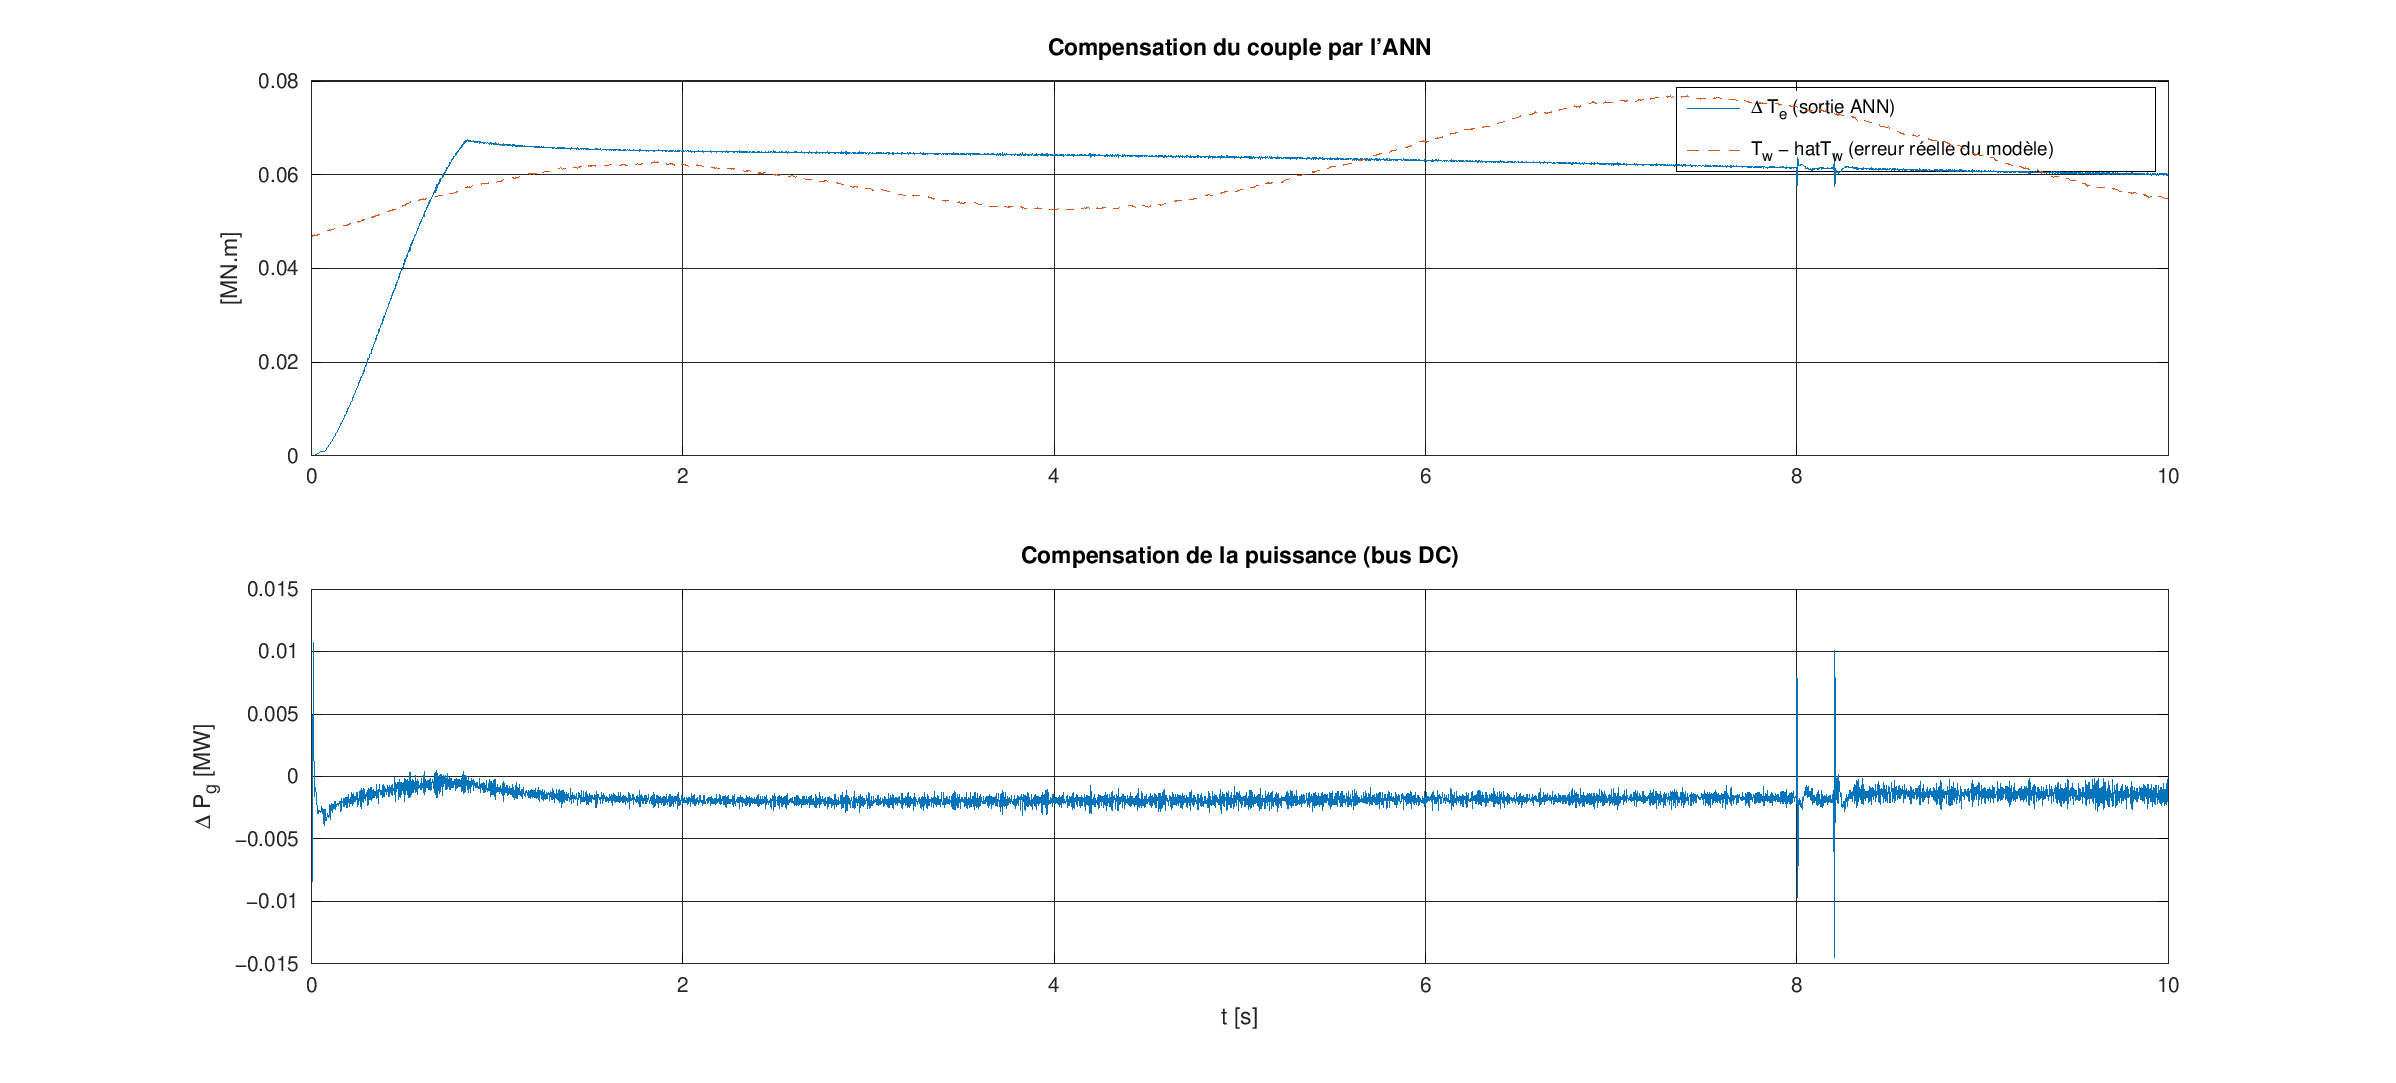
\includegraphics[width=0.95\textwidth]{fig_ann.png}
\caption{الأعلى: مخرج الشبكة $\Delta T_e$ (أزرق) والخطأ الحقيقي للنموذج $T_w-\hat T_w$ (برتقالي).}
\end{figure}
في اختبار المتانة، النموذج يقلّل $T_w$ بـ $10\%$، أي بين $0{,}05$ و $0{,}077\ \mathrm{MN\cdot m}$.
الشبكة \textbf{لا تعرف هذا}. ومع ذلك، في أقل من ثانية، يصير $\Delta T_e \approx 0{,}065\ \mathrm{MN\cdot m}$،
أي تقريباً متوسط الخطأ الحقيقي. لقد «اكتشفت» الخطأ من خلال أخطاء السرعة فقط.
الجزء المتغيّر ببطء يصحّحه الجزء التكاملي لقانون التسطيح.

% =====================================================================
\section{المحاكاة: كيف يحسب الحاسوب؟}
% =====================================================================

\paragraph{الفكرة.} الحاسوب لا يستطيع حلّ المعادلات «مرة واحدة». يتقدّم بخطوات صغيرة جداً
($T_s = 0{,}0001\ \mathrm{s}$):
\[
x(t+T_s) \approx x(t) + T_s\cdot\frac{dx}{dt}
\]
«القيمة الجديدة = القديمة + الخطوة $\times$ سرعة التغيّر». هذه طريقة \fr{Euler}. نحن نستعمل طريقة أدقّ
(\fr{Runge-Kutta 4})، تحسب سرعة التغيّر 4 مرات داخل الخطوة وتأخذ المتوسط.

\paragraph{ما يحدث في كل خطوة (في السكريبت \fr{PMSG\_Plate\_PBC\_ANN.m}).}
\begin{enumerate}
\item نقرأ الريح وجهد الشبكة.
\item \textbf{(a)} الـ \fr{MPPT}: نحسب $\Omega^*$.
\item \textbf{(b)} التسطيح، السرعة: نحسب $T_e^*$ ثم $i_{sq}^*$.
\item \textbf{(c)} السلبية، المقوّم: نحسب $\bv{v}_s^*$.
\item \textbf{(d)} التسطيح، الحافلة: نحسب $P_g^*$ ثم $i_{gd}^*$.
\item \textbf{(e)} السلبية، المموّج: نحسب $\bv{v}_i^*$.
\item \textbf{(f)} الشبكة العصبونية: تتعلّم وتحسب $\Delta T_e, \Delta P_g$ للخطوة القادمة.
\item نطبّق الجهود على النموذج، ونتقدّم بخطوة واحدة (\fr{RK4}).
\end{enumerate}
نكرّر هذا $100\,000$ مرة لنحاكي $10$ ثوانٍ.

% =====================================================================
\section{قراءة النتائج}
% =====================================================================

\begin{figure}[h]
\centering
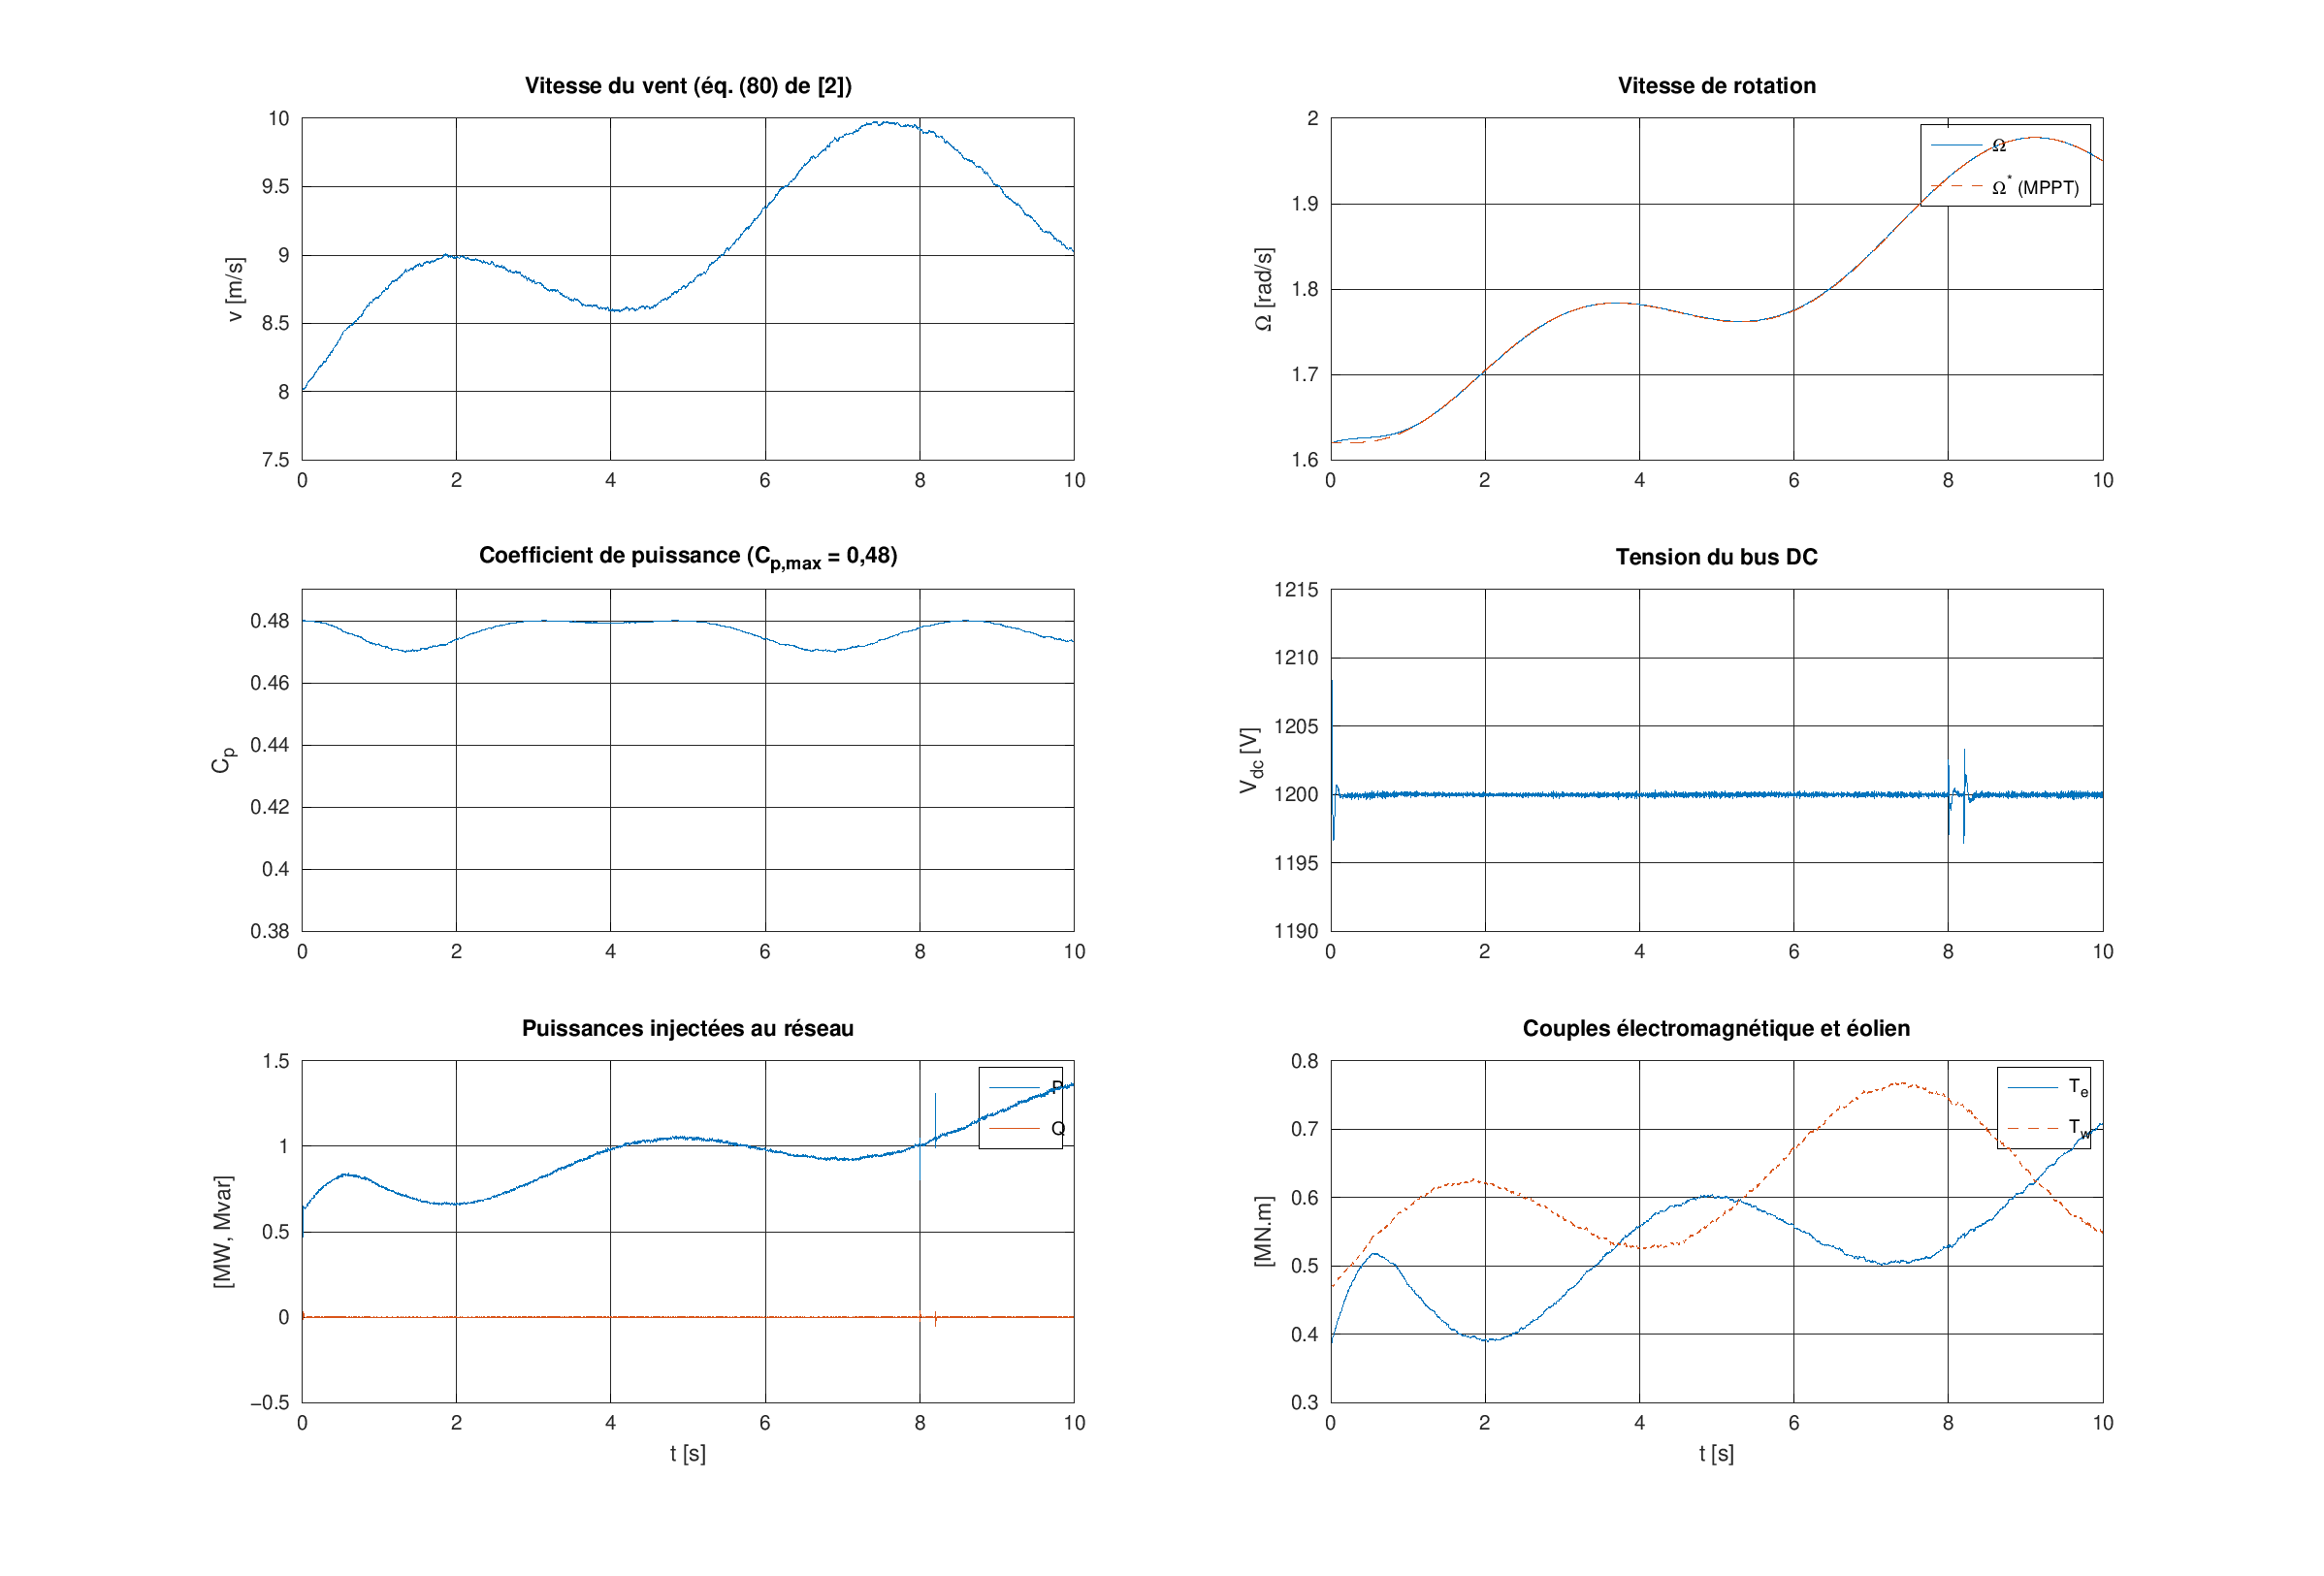
\includegraphics[width=\textwidth]{fig_ensemble.png}
\caption{اختبار المتانة مع الشبكة العصبونية.}
\end{figure}
\begin{itemize}
\item \textbf{الريح} (أعلى اليسار): نفس ريح المقال.
\item \textbf{السرعة}: $\Omega$ فوق $\Omega^*$ تماماً، فالـ \fr{MPPT} يعمل.
\item \textbf{$C_p$}: بين $0{,}47$ و $0{,}48$، قريب جداً من الأقصى.
\item \textbf{$V_{dc}$}: ثابت على $1200\ \mathrm{V}$. عند $t=8\ \mathrm{s}$ ينخفض جهد الشبكة بـ $20\%$
(\fr{creux de tension})، فيتحرّك $V_{dc}$ بحوالي $\pm10\ \mathrm{V}$ ويرجع في أقل من $0{,}3\ \mathrm{s}$.
\item \textbf{القدرة}: $P$ تتبع الريح، و $Q = 0$.
\item \textbf{العزوم}: $T_e$ يتبع $T_w$ بتأخير، وهذا طبيعي بسبب عطالة التوربينة.
\end{itemize}

\begin{center}
\begin{tabular}{lccc}
\toprule
المؤشّر (اختبار المتانة) & بدون \fr{ANN} & مع \fr{ANN} & التحسّن\\
\midrule
خطأ السرعة \fr{IAE} & $0{,}0109$ & $0{,}0067$ & $-39\%$\\
خطأ الحافلة \fr{ISE} & $1{,}30$ & $1{,}16$ & $-11\%$\\
أقصى انحراف لـ $V_{dc}$ & $10{,}4\ \mathrm{V}$ & $10{,}4\ \mathrm{V}$ & نفسه\\
$C_p$ المتوسط & $0{,}476$ & $0{,}476$ & نفسه\\
\bottomrule
\end{tabular}
\end{center}
\textbf{IAE} = مجموع القيمة المطلقة للخطأ عبر الزمن. \textbf{ISE} = مجموع مربّع الخطأ. كلّما صغر، كان التتبّع أفضل.

\begin{khulasa}
\Khulasa
الشبكة العصبونية، بدون تغيير أيّ معامل في التحكّم الأساسي، تقلّل خطأ السرعة بـ $39\%$ عندما يكون
النموذج خاطئاً. والطاقة المنتجة لا تتغيّر، لأن التحسّن في دقّة التتبّع وليس في كمية الطاقة.
\end{khulasa}

% =====================================================================
\section{أسئلة قد يطرحها الأستاذ (مع أجوبتها)}
% =====================================================================

\begin{enumerate}
\item \textbf{لماذا \fr{PMSG} وليس \fr{DFIG}؟}
لأنه يعمل بدون علبة سرعات (أقل صيانة)، وبدون فرش، ومردوده جيّد. ثمنه أنه يحتاج محوّلاً بكامل القدرة.

\item \textbf{لماذا $i_{sd}^* = 0$؟}
لأن العزم يأتي فقط من $i_{sq}$ (الآلة بأقطاب ملساء $L_d=L_q$). أيّ تيار $i_{sd}$ يسبّب ضياعاً بدون فائدة.

\item \textbf{لماذا التسطيح للحلقات الخارجية؟}
لأن معادلاتها بسيطة وقابلة للقلب (عمود ميكانيكي، توازن طاقة). التسطيح يستعمل النموذج ليتوقّع، فيكون
أسرع من \fr{PI} الذي ينتظر الخطأ.

\item \textbf{لماذا الطاقة وليس الجهد كمخرج مسطّح للحافلة؟}
لأن $\dot W = P_{msc} - P_{gsc}$ معادلة خطّية في القدرة، بينما معادلة $V_{dc}$ غير خطّية (فيها $1/V_{dc}$).

\item \textbf{لماذا السلبية للتيارات؟}
لأن معادلات التيارات لها بنية طاقوية (حدّ التزاوج بدون عمل). السلبية تحترم هذه البنية، وتعطي برهان
استقرار بسيط ($dH/dt\le0$).

\item \textbf{ما الفرق بين شبكتنا والشبكات «العادية»؟}
الشبكات العادية تُدرَّب مسبقاً على بيانات (\fr{offline}). شبكتنا تتعلّم \textbf{أثناء التشغيل}
(\fr{online})، وأوزانها متغيّرات تتطوّر مع النظام.

\item \textbf{لماذا تضيف الشبكة تصحيحاً بدل أن تغيّر المعاملات؟}
لكي يبقى التحكّم الأساسي ومعاملاته وبرهان استقراره كما هي. الشبكة «تساعد» فقط، وإذا أطفأناها يعمل
النظام بالتحكّم الأساسي.

\item \textbf{ما معنى \fr{UUB}؟}
الخطأ لا يذهب بالضرورة إلى الصفر تماماً، لكنه يدخل منطقة صغيرة حول الصفر ولا يخرج منها.

\item \textbf{هل البارامترات حقيقية؟}
بارامترات الآلة والحافلة والشبكة من مقال منشور (\fr{Hasan \& Shatil, AJSE 2021}). بارامترات التوربينة من
الأستاذ. فقط $J$ و $B$ و $R_f$ فرضيات.

\item \textbf{ما حدود العمل؟}
لا يوجد تحكّم في زاوية الشفرات (الريح أقل من الاسمية)، والـ \fr{PLL} مثالية، والنتائج الرئيسية بالنموذج
المتوسط، وقانون السرعة يستعمل الريح المقاسة.
\end{enumerate}

% =====================================================================
\section*{ملحق: قاموس المصطلحات}
% =====================================================================
\begin{center}
\begin{tabular}{lll}
\toprule
العربية & \fr{Français} & \fr{English}\\
\midrule
مولّد متزامن بمغانط دائمة & \fr{machine synchrone à aimants permanents} & \fr{PMSG}\\
مقوّم / مموّج & \fr{redresseur / onduleur} & \fr{rectifier / inverter}\\
تعديل عرض النبضة & \fr{MLI} & \fr{PWM}\\
الحافلة المستمرة & \fr{bus continu (DC)} & \fr{DC link}\\
معامل القدرة الهوائي & \fr{coefficient de puissance $C_p$} & \fr{power coefficient}\\
نسبة السرعة الطرفية & \fr{vitesse spécifique $\lambda$} & \fr{tip-speed ratio}\\
تتبّع نقطة القدرة القصوى & \fr{MPPT} & \fr{maximum power point tracking}\\
التحكّم بالتسطيح & \fr{commande par platitude} & \fr{flatness-based control}\\
المخرج المسطّح & \fr{sortie plate} & \fr{flat output}\\
التحكّم بالسلبية & \fr{commande passive (PBC)} & \fr{passivity-based control}\\
حقن التخميد & \fr{injection d'amortissement} & \fr{damping injection}\\
دالة التخزين / ليابونوف & \fr{fonction de stockage / de Lyapunov} & \fr{storage / Lyapunov function}\\
شبكة عصبونية & \fr{réseau de neurones (ANN)} & \fr{artificial neural network}\\
الوزن / الانحياز & \fr{poids / biais} & \fr{weight / bias}\\
الطبقة المخفية & \fr{couche cachée} & \fr{hidden layer}\\
الانتشار العكسي & \fr{rétropropagation} & \fr{backpropagation}\\
المنطقة الميتة & \fr{zone morte} & \fr{dead-zone}\\
محدود نهائياً بانتظام & \fr{uniformément ultimement borné} & \fr{UUB}\\
انخفاض الجهد & \fr{creux de tension} & \fr{voltage dip}\\
\bottomrule
\end{tabular}
\end{center}

\end{document}
